
In Section~\ref{sec:fase-methodology}, we explained that carriers are found by searching for a shape that shifts by $f_\Delta$ when $f_{alt}$ changes by $f_\Delta$. However, visual comparison of numerous recorded spectra across a wide range of frequencies would be tedious and error prone. Equations~\ref{eq:filter_top} and ~\ref{eq:filter_detailed} a simplified and easily-implementable heuristic for finding side-bands whose shifts in frequency correspond to shifts in $f_{alt}$. For a given harmonic $h$ of $f_{alt}$, the function $F_h(f)$ is intended to have a large value for a frequency that corresponds to a activity-modulated carrier. We compute this score as 
\begin{equation}
F_h(f) = \prod_i F_{i,h}(f)
\label{eq:filter_top}
\end{equation} 
where $F_{i,h}(f)$ is a sub-score for the $i$-th recorded spectrum ($i$-th $f_{alt}$). This subscore is computed as 
\begin{equation}
F_{i,h}(f) = \frac{SP_i(f+h\cdot f_{alt_i})}{\frac{1}{N-1}\sum_{j \neq i} SP_j(f+h\cdot f_{alt_j})}.
\label{eq:filter_detailed}
\end{equation}
This function first appropriately shifts $SP_i(f)$, the spectrum captured with the microbenchmark active at alternation frequency $f_{alt_i}$, so a side-band signal at $f_c+h\cdot f_{alt_i}$ gives a peak in $F_{i,h}$ at the carrier frequency $f=f_c$, i.e. we score the side-band signals, but the sub-score is ``reported'' at $f_c$.

The value of the sub-score is computed by normalizing the strength of the side-band signal in this spectrum by the average of the other \hskip2pt $N\hskip-2pt -\hskip-2pt 1$ \hskip2pt $f_{alt_j}$ spectra. For side-band signals that do shift in frequency as $f_{alt}$ changes, the sub-score for a particular $i$ will be larger than 1 because the side-band signal is stronger at the $f_c+f_{alt}$ frequency in this spectrum. At the exact same frequency in at least some of the other spectra, however, the signal will not be as strong because these spectra have peaks at $f_{alt_j}$ and so their side-band signal is at a different frequency. In contrast, a strong signal that does not shift in frequency as $f_{alt}$ changes will stay at the same frequency in the other spectra, so the normalization will produce a score close to 1. The overall score $F_h(f)$ multiplies the sub-scores, so the overall score is close to 1 if no $f_{alt}$-induced frequency shifting occurs. If each $i$-th spectrum has side-band signals at $f_{alt_i}$, the frequency-shifted sub-scores will align producing a very large value for the carrier frequency. Finally, if only some side-band signals are present (one or a few may be ``buried'' by some unrelated signal), the overall score will be weakened because each obscured $f_{alt_i}$ side-band will have a sub-score close to 1, but the remaining sub-scores will still increase the overall score significantly above 1. Overall, this heuristic produces large peaks at frequencies of modulated carriers and is almost completely flat at all other frequencies. Figure~\ref{filter} shows the heuristic function's output for the carriers shown in Figures~\ref{mem_refresh_zoom}~and~\ref{core_reg_zoom}. Figure~\ref{lx61_mem_ssc_c} shows the heuristic function for the DRAM clock signal shown in Figure~\ref{lx61_mem_ssc_b}. FASE clearly does detect such modulated signals though it reports the clock as two separate carriers at the edges of the spread out clock signal.

\begin{figure}[htb]
  \centering
    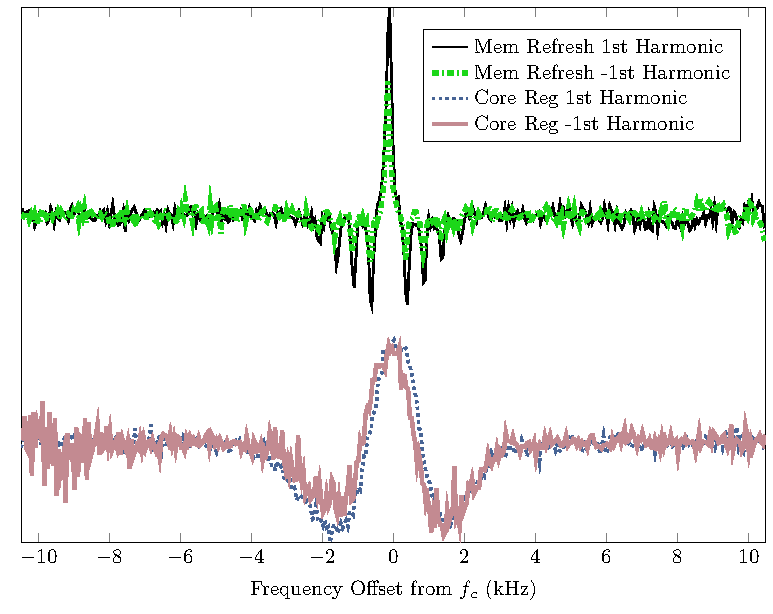
\includegraphics[width=5in]{../fase/Data/filter.pdf}%
  \caption{Output of the heuristic for the 1st and -1st harmonics of $f_{alt}$ for two carriers.}%
  \label{filter}
\end{figure}

\begin{figure}[htb]
\centering
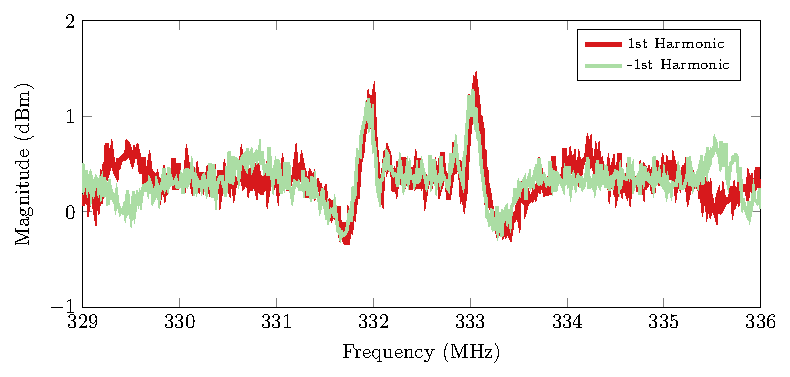
\includegraphics[trim=0.1in 0.10in 0.1in 0.09in,clip,width=5in]{../fase/Data/lx61_mem_ssc_c.pdf}%
\caption{Output of the heuristic function for an SSC DRAM clock signal.}%
\label{lx61_mem_ssc_c}
\end{figure}

The heuristic function provides a good indicator of the frequencies at which modulated carriers are likely to occur. The next step in automating FASE is to find the peaks in the $H_h(f)$ output. To do this, we sort the peaks by their prominence and keep only those with prominence greater than 1.5dB. Except for the highest peak in a spectrum, every peak sits within a valley bounded on the left and right by two higher peaks. We calculate the prominence of a peak as the magnitude of the peak in the valley minus the magnitude at the lowest point in these valley. Ideally, finding the peaks in the heuristic function would be sufficient to find all the modulated carriers. However, for realistic spectra not all peaks are caused by unintentional modulation. For example, a transient signal occurring in one of the 5 recorded spectra can cause variation in $H_h(f)$ which might be mistaken for a modulated carrier (i.e. a false positive). In such cases, the output of the heuristic alone is not sufficient to reliably report AM carriers, and some additional processing is needed.

\begin{figure}[htb]
\centering
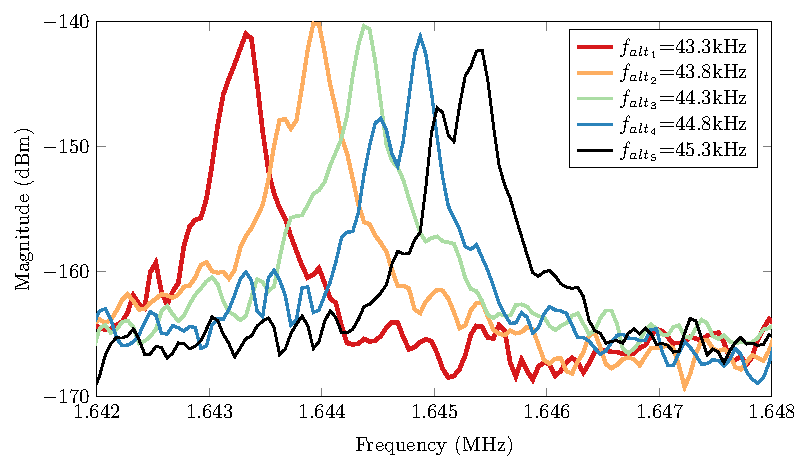
\includegraphics[width=5in]{../eucap_fase/Drawing/sb_good.pdf}
\caption{Easy to detect spectral pattern at $f_c+f_{alt_i}$ caused by an AM carrier at $f_c$=1.6MHz on the Samsung Galaxy S5 smartphone.}
\label{sb_good}
\end{figure}

Also, recall that we need to search for the spectral patterns created by FASE for 10 different harmonics ($h=-5,...-1,1,...,5$). Furthermore, the negative and positive harmonics are ``flipped.'' In other words, each peak in $H_h(f)$ is caused by a set of $N$ peaks in the spectra spaced evenly by $hf_\Delta$ as shown in Figure~\ref{sb_good}. This spectral pattern occupies a smaller or larger frequency range depending on its respective harmonic. Also, the positive harmonics (right sideband) have the $f_{alt_1}$ peak on the left and the $f_{alt_N}$ peak on the right, but the order of the peaks is reversed for the negative harmonics (left sideband). To simplify processing, when we find a peak in the heuristic function, we create a ``normalized frame.'' This normalized frame flips the signals for the negative harmonics so that the order of the peaks is the same as for the positive harmonics, and also scales the x-axis so that we have the same number of frequency points regardless of the detected harmonic $h$. After this normalization, each frame can be processed the same regardless of its harmonic. To filter out false positives, we extract relevant features from each frame and use a neural network to reduce the number of reported false positives. The extracted features and neural network are described in~\cite{wang2016}.

We evaluated the effectiveness of this automated procedure by testing it on spectra from the desktop, laptops, and smartphone systems in Table~\ref{fase_pc_specs}. The desktop and laptop measurements used a magnetic loop antenna (AOR LA400) at a distance of 30 cm as shown in on the left of Figure~\ref{sec:fase-setup}. The generally weaker smartphone EM emanations were recorded using a small loop probe with 20 turns and a 4 mm radius shown on the right of Figure~\ref{fase_auto_setup}. The smartphone probe was placed directly above the screen over the area where the induced baseband signal had the largest magnitude. The smartphone spectra were measured from 0 to 10 MHz and the computer spectra were measured from 0 to 4 MHz. We used $f_{alt_1}$ = 43.3 kHz and $f_\Delta$ = 500 Hz with five alternation frequencies (i.e. $f_{alt_1}$ through $f_{alt_1}+4f_\Delta$) and the LDM/LDL1 (DRAM memory) and LDL2/LDL1 (processor) activities. The benchmarks were run on the laptop and desktop systems as single-threaded Windows 7 32-bit user mode console applications, and were run on the smartphones as normal Android applications. When possible all unrelated programs and activities were disabled, CPU frequency scaling was disabled, and screens were turned off. The spectra were recorded using a spectrum analyzer (Agilent MXA N9020A). 

\begin{table}[htbp]%
  %\small%
  \footnotesize %
  \centering%
    \begin{tabular}{cccc}%
    \toprule
    \textbf{Type} & \textbf{Device} & \textbf{Processor} & \textbf{Carriers Found}\\
    \midrule
    %carriers found is not systematic, manual total counted
    Desktop & Dell & Intel i7 & 20 \\
    Laptop & HP & AMD Turion X2 & 7 \\
    Laptop & Lenovo & Intel Core 2 Duo & 6 \\
    Phone & Samsung Galaxy S5 & Snapdragon 801 & 7 \\
    Phone & LG P705 & Snapdragon S1 & 6 \\
    Phone & Motorola Moto G & Snapdragon 400 & 2 \\
    \bottomrule
    \end{tabular}%
  \caption{Devices for the automated FASE measurements.}%
  \label{fase_pc_specs}%
\end{table}%

\begin{figure}[htb]
\centering
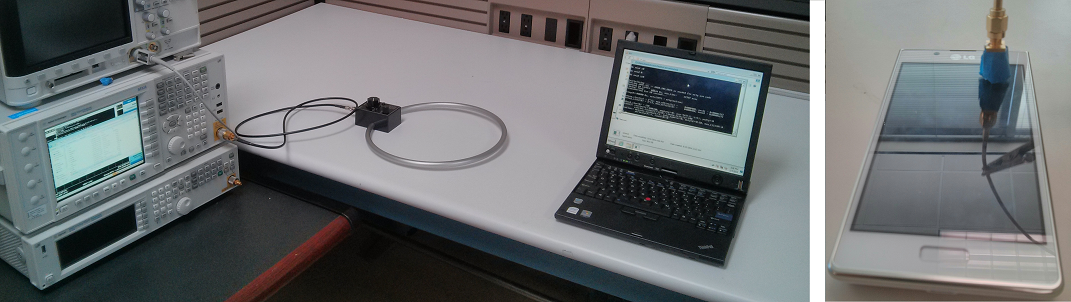
\includegraphics[width=5in]{../eucap_fase/setup.png}
\caption{Setup for the automated FASE measurements.}
\label{fase_auto_setup}
\end{figure}


%MISSED  TRUEP FALSEN FALSEP  TRUEN
%     9    129     11     21    199
%total = 149, missed =   0.06%, algo: total = 360, correct =   0.91%

We tested the six devices in Table~\ref{fase_pc_specs}, with two measurements per device (one for LDM/LDL1 and one for LDL2/LDL1). To test the accuracy of the algorithm we began by visually inspecting all the spectra and manually listing any detected signals. Determining whether a $f_{alt_i}$ spectral pattern for a given AM carrier is detectable is subjective due to the noisy and crowded nature of the spectrum. For our testing, we included only those spectral patterns where at least 3 of the 5 $f_{alt_i}$ peaks were visible. By this criteria, we found 149 spectral patterns in total by visual inspection. Nine of these patterns did not create peaks above the heuristic function's detection threshold. The heuristic functions $H_h(f)$ had 360 peaks above the prominence threshold (i.e. 360 indications of possible modulation). Frames were created for these 360 cases and tested using the neural network. The neural network predicted whether the frames corresponded to actual unintentional modulation with 91\% accuracy.

\begin{figure}[htb]
\centering
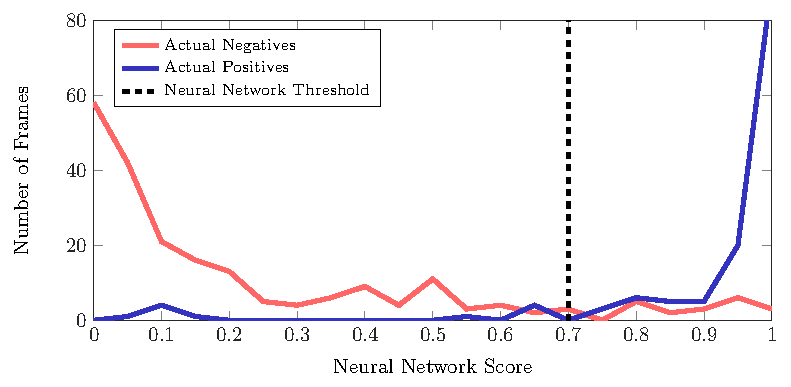
\includegraphics[width=5in]{../eucap_fase/Drawing/nn_dist.pdf}
\caption{Distribution of the neural network scores.}
\label{nn_dist}
\end{figure}

Figure~\ref{nn_dist} shows distributions of the neural network's score for the tested frames. In this figure, the blue distribution contains the 140 frames which occurred at frequencies where generated spectral patterns were caused by modulated carriers (i.e. actual positives), and the red distribution indicates the 220 frames that occurred at frequencies where no modulation was found via visual inspection (i.e. actual negatives). The dotted black line indicates the neural network threshold used. The neural network predicted all the frames to the right of this line as positive, meaning that the actual positives to the right of this line are true positives and the actual negatives to the right of this line are false positives. Similarly, false negatives and true negatives occur to the left of this line. 

Many of the true positive frames resemble the example shown in Figure~\ref{sb_good} and were easily classified as positives. Similarly, many of the true negatives were caused by random variations in the spectra and were easily classified as negatives. However, the remaining 9\% of the frames were incorrectly predicted. In some such frames, several of the $f_{alt_i}$ peaks were obscured or misshapen. For example, the frame shown in Figure~\ref{sb_hard} was correctly predicted, but had a score near the neural network threshold. As the spectral pattern's peaks became further obscured and as the shapes of the peaks became less regular, the frames were more likely to be incorrectly predicted (i.e. false negatives). Similarly, false positives occurred where random variations in the spectra create patterns that resemble the spectral patterns generated by AM modulation.

\begin{figure}[htb]
\centering
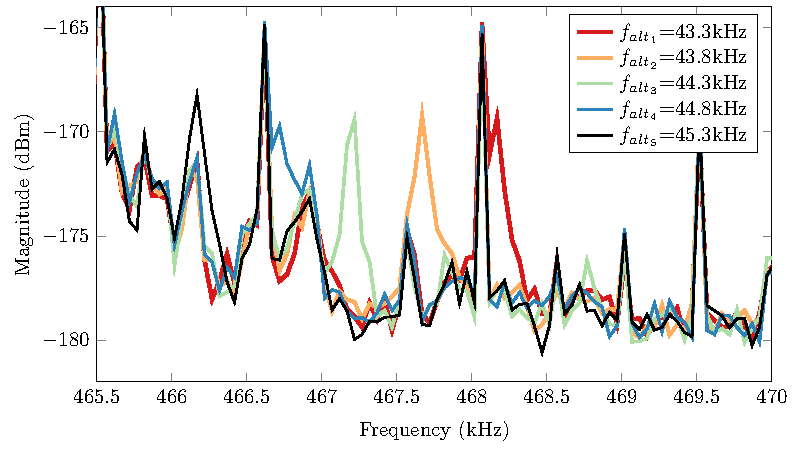
\includegraphics[width=5in]{../eucap_fase/Drawing/sb_hard.pdf}
\caption{Difficult to detect frame at $f_c-f_{alt_i}$ for an AM carrier at $f_c$=511kHz on the Lenovo laptop.}
\label{sb_hard}
\end{figure}

% samsung s5 circuit descriptions: 
% http://www.techinsights.com/teardown.com/samsung-galaxy-S5-teardown/
% this is where the battery connects to the phone, so I'm assuming voltage regulator
%https://www.ifixit.com/Guide/LG+Optimus+L7+P705+Charger+Port+Replacement/33461

The unintentional AM carriers found for the desktops and laptops were caused by voltage regulators, memory clocks, and memory refresh commands. For the smartphones, several carriers were found to be caused by voltage regulators. The remainder of the carriers found on the smartphones could be traced to particular IC packages or modules and were determined to be modulated only by memory activities. However, smartphones integrate many system components into System on Chip (SoC) modules and often use Package on Package (PoP) technology to integrate both the processor and memory into the same package and little information is publicly available describing these components. More information would be needed to definitively determine the circuits and mechanisms modulating these carriers.

